% File template.tex
%
% This is a template file for the LHCSki 2016 workshop

\documentclass{article}
\usepackage{authblk}
\usepackage{graphicx}
\usepackage{verbatim}
\usepackage{hyperref}
\usepackage{amsmath,amssymb}

\newcommand{\MET}{${\mathrm{E_{T}^{miss}}}$}
\newcommand{\pt}{${\mathrm{p_{T}}}$}
\newcommand{\ttbar}{${\mathrm{t\bar{t}}}$}
\newcommand{\HT}{$\mathrm{H_T}$}
\newcommand{\MJ}{$\mathrm{M_J}$}
\newcommand{\MT}{$\mathrm{M_T}$}
\newcommand{\MTtwo}{$\mathrm{M_{T2}}$}
\newcommand{\LT}{$\mathrm{L_T}$}
\newcommand{\dphiwl}{$\mathrm{\Delta\Phi(W, \ell)}$}
\newcommand{\njets}{$\mathrm{N_{jets}}$}
\newcommand{\nbtags}{$\mathrm{N_{b-tags}}$}
\newcommand{\mll}{$\mathrm{M_{\ell\ell}}$}

\begin{document}
\newcommand{\sessionday}[1]{\iffalse#1\fi} %% please leave that line
\newcommand{\speaker}{\author}

\sessionday{Tuesday} %% please insert day of your talk here, e.g. monday
\title{Searches for supersymmetry at CMS in leptonic final states with 13 TeV Data}

% the authors, in the "right" order
%% \author[1]{Firstname, Lastname}
%% % the speaker will be underlined
\speaker[1]{C. Vince Welke on behalf of the CMS Collaboration}
%% \author[]{}

%% \author[1,2]{C. Vince, Welke}
%% \affil[1]{CMS}
\affil[1]{University of California - San Diego, La Jolla, California}

\maketitle

\abstract{
  The CMS SUSY program is very active in performing searches with the 13 TeV data including multiple analyses done in regions with leptonic final states.
  The results of these analyses are used to expand the reach of the searches done by CMS at 8 TeV and additionally to investigate two excesses seen in run I,
  namely a 2.6 sigma excess seen by CMS and a 3.0 sigma excess seen by ATLAS.
  These excesses were observed in two separate signal regions both having final states of at least 2 opposite sign same flavor leptons, jets, and \MET.}

Supersymmetry (SUSY)~\cite{SUSYPrimer} is an extension to the standard model that can explain some of the open problems in physics such as
a solution the hierarchy problem as well as providing potential candidates for dark matter.
Searches for SUSY are performed by the CMS collaboration in a variety of final states,
including searching for processes with leptons (e or $\mu$) in the final state.
Simplified models~\cite{sms} are used to interpret results of these searches, where two examples are shown in figure~\ref{fig:SMS}.
On the left is a diagram of a gauge mediated SUSY breaking (GMSB) model with a massless gravitino as the lightest SUSY particle (LSP).
In this model, gluinos are pair produced, and each decays to a pair of quarks and a neutralino, which subsequently decays to a Z boson and a gravitino.
Another model showing direct stop production with one of the stops eventually
decaying to a top that decays leptonically is shown on the right.
The results presented in these proceedings focus on direct squark and gluino production.
In all of the following results, no significant deviation from the SM was observed,
and limits are set on the upper limit of the cross section of simplified models at the 95\% level using the CLs method~\cite{Junk:1999kv,Read:2002hq}.

\begin{figure}[!htb]
\begin{center}
\begin{tabular}{cc}
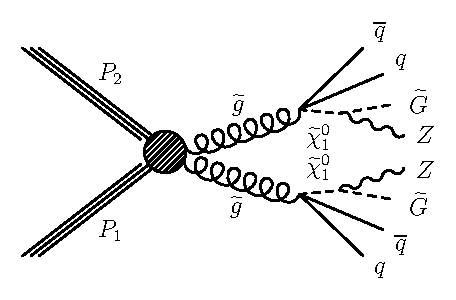
\includegraphics[width=0.4\textwidth]{intro/Feynman_graph_T5ZZgmsb.pdf} &
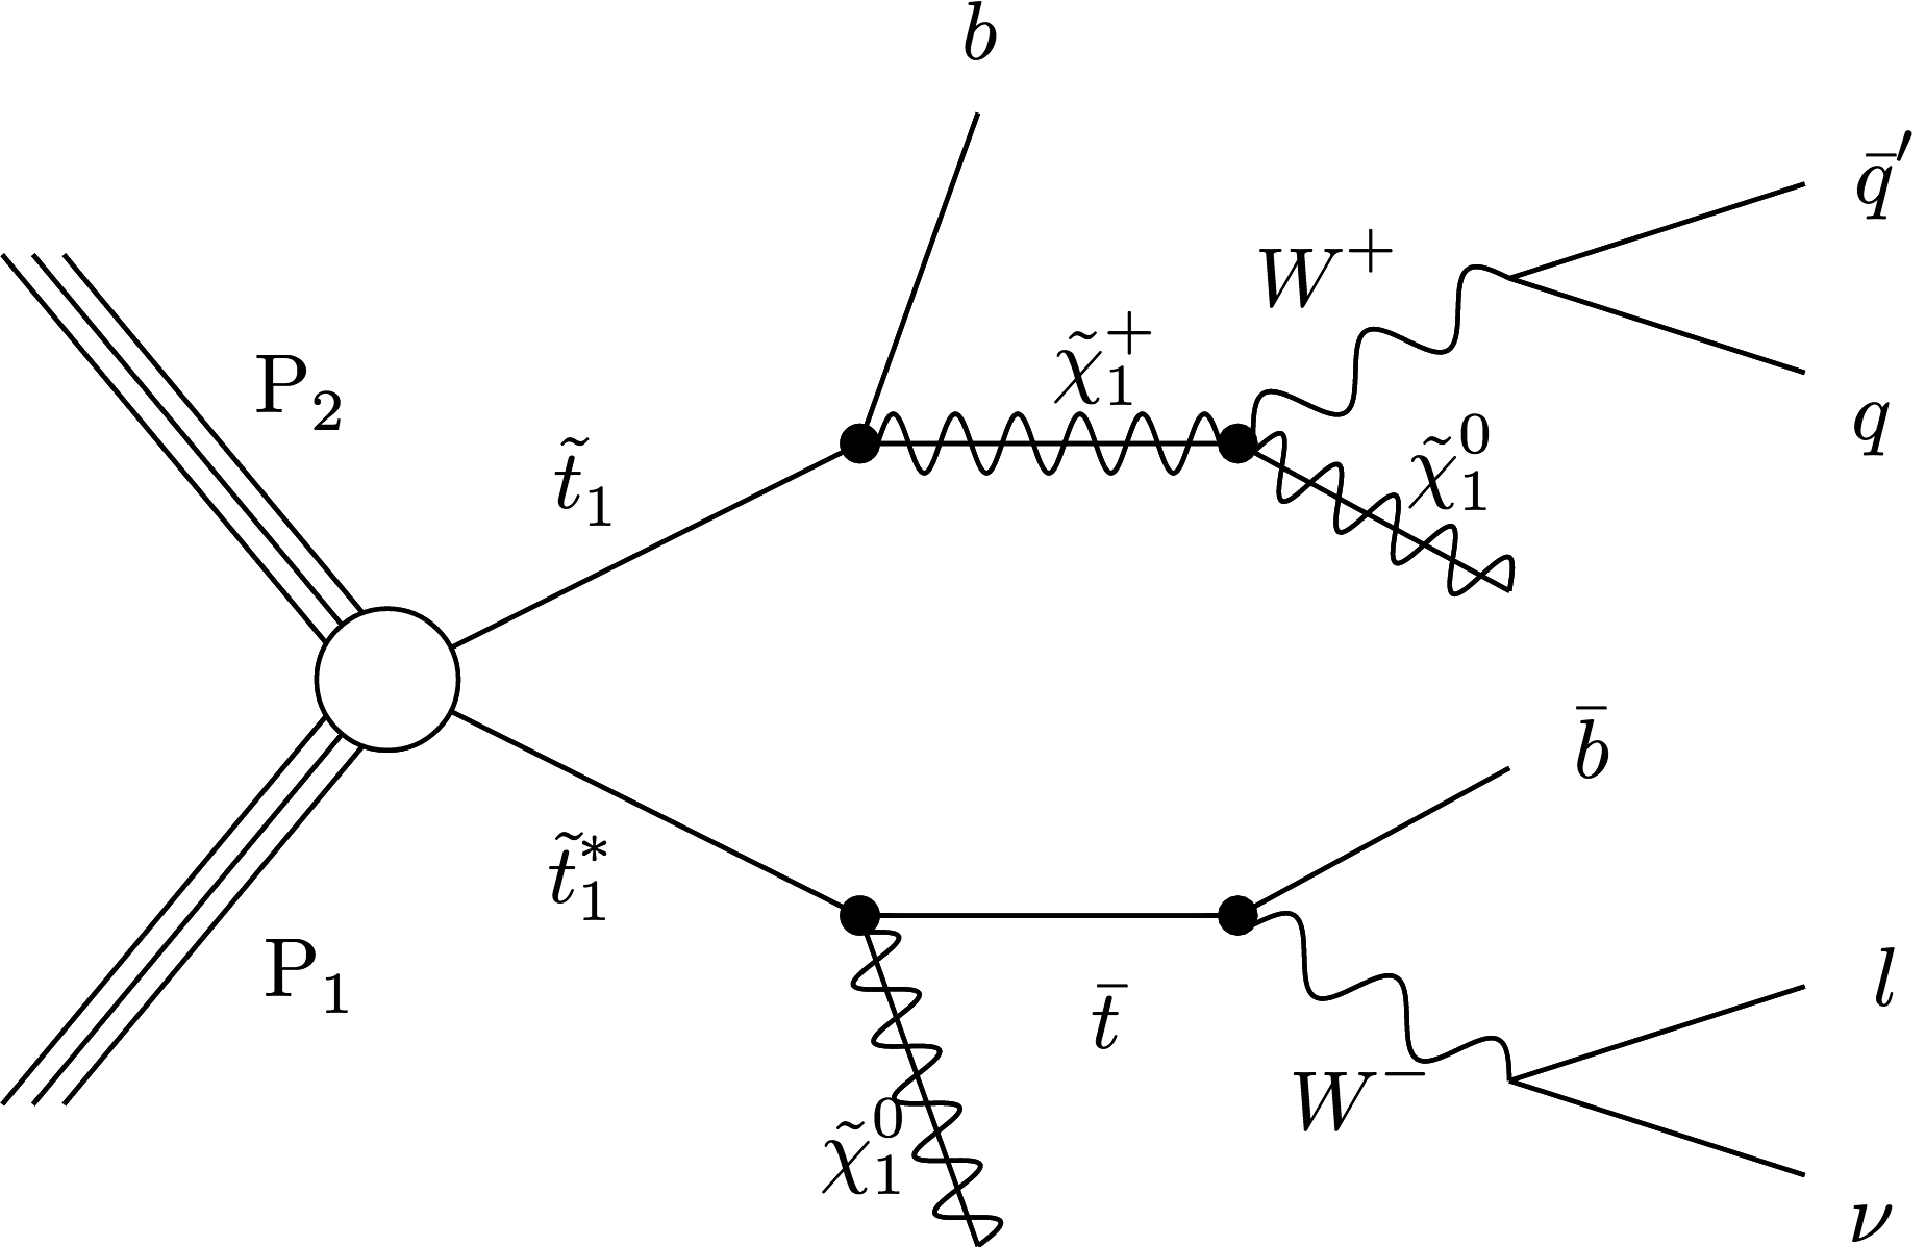
\includegraphics[width=0.4\textwidth]{intro/T2tt.pdf}
\end{tabular}
\caption{
\label{fig:SMS}
Diagrams showing different SUSY processes which may contain leptons in the final state are shown in this figure.
On the left, gravitinos are pair-produced, where each eventually decays to a Z boson, two quarks, and a gravitino.
On the right, stops are pair-produced, where one leg eventually decays to a top and a neutralino where the top decays leptonically.
}
\end{center}
\end{figure}

The SUSY analyses performed by CMS share very similar object definitions for electrons, muons, and jets. 
They are then grouped by the number of leptons in the final state,
and for analyses with at least two leptons,
they are categorized according to the charge of the two leptons with the highest \pt\
in same-sign, or opposite-sign final states.
Additionally, a large range of topologies are targeted by varying the following event variables:
Visible energy:
\HT\ is the scalar sum of the jet \pt\ in the event.
\MJ\ is the sum of reclustered jets; this is explained in more detail in the \MJ\ analysis section.
Invisible energy:
\MET\ is the magnitude of the vector sum of all the objects in the event, which is corrected to be consistent with the corrections applied to jets.
\MT\ is the transverse mass made using a lepton and the \MET\ vector.
\MTtwo\ is the stransverse mass, which is made from two visible objects and the \MET\ vector; This is explained in more detail in the 1-lepton stop search section.
\dphiwl\ is the difference in $\phi$ between the lepton and the W-candidate in the 1-lepton inclusive analysis.
\LT\ is defined as the vector sum of the lepton and the \MET\ in the 1-lepton inclusive analysis.
Jet multiplicity and flavor content: \njets\ and \nbtags.

In the analyses with exactly one lepton, three separate searches are performed.
In the first search, a search for direct stop pair production~\cite{1lstop2015}, the signal region is defined by having
exactly 1 lepton, at least 2 jets with at least one of the jets passing the criteria to be tagged as a b-jet, and \MET\ $>$ 250 GeV.
In order to suppress backgrounds from ttbar, a cut is then made on $\mathrm{M_{T2W}}$,
which is an \MTtwo-like variable that uses the b-jets and leptons as visible objects, and has a kinematic cut-off at the top mass.
After the cuts are applied, the largest background comes from SM \ttbar\ to dilepton where one of the leptons is lost leading to increased \MET\ in the event.
The results of this analysis increase the sensitivity to stop production for signal models with a stop mass of 750 GeV,
which is an improvement on the previous result which was sensitive to models with a stop mass up to 650 GeV.
%% The yields in data overlaid on the background predictions can be seen on the left in figure~\ref{fig:1lstopresults},
%% and the cross section upper limit is shown as a function of the stop mass on the x-axis and LSP mass on the y-axis.

%% \begin{figure}[!htb]
%% \begin{center}
%% \begin{tabular}{cc}
%% 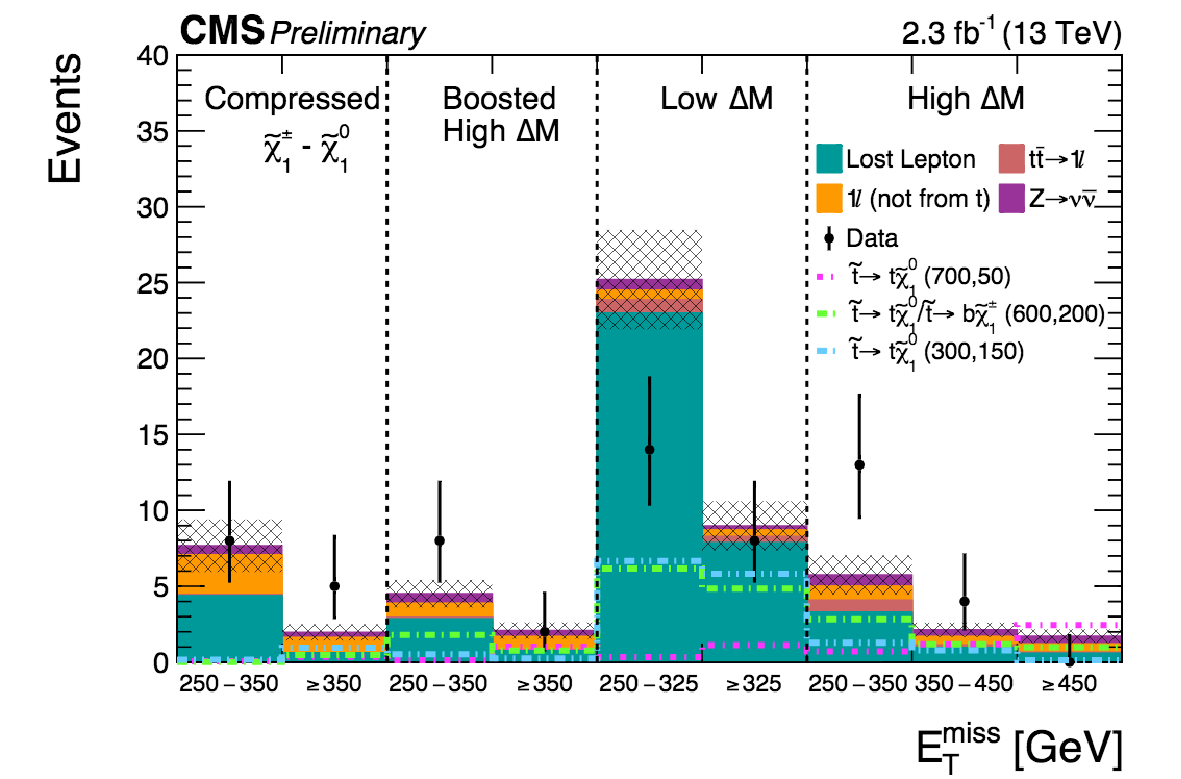
\includegraphics[width=0.4\textwidth]{1lstop/results_summary.pdf} &
%% 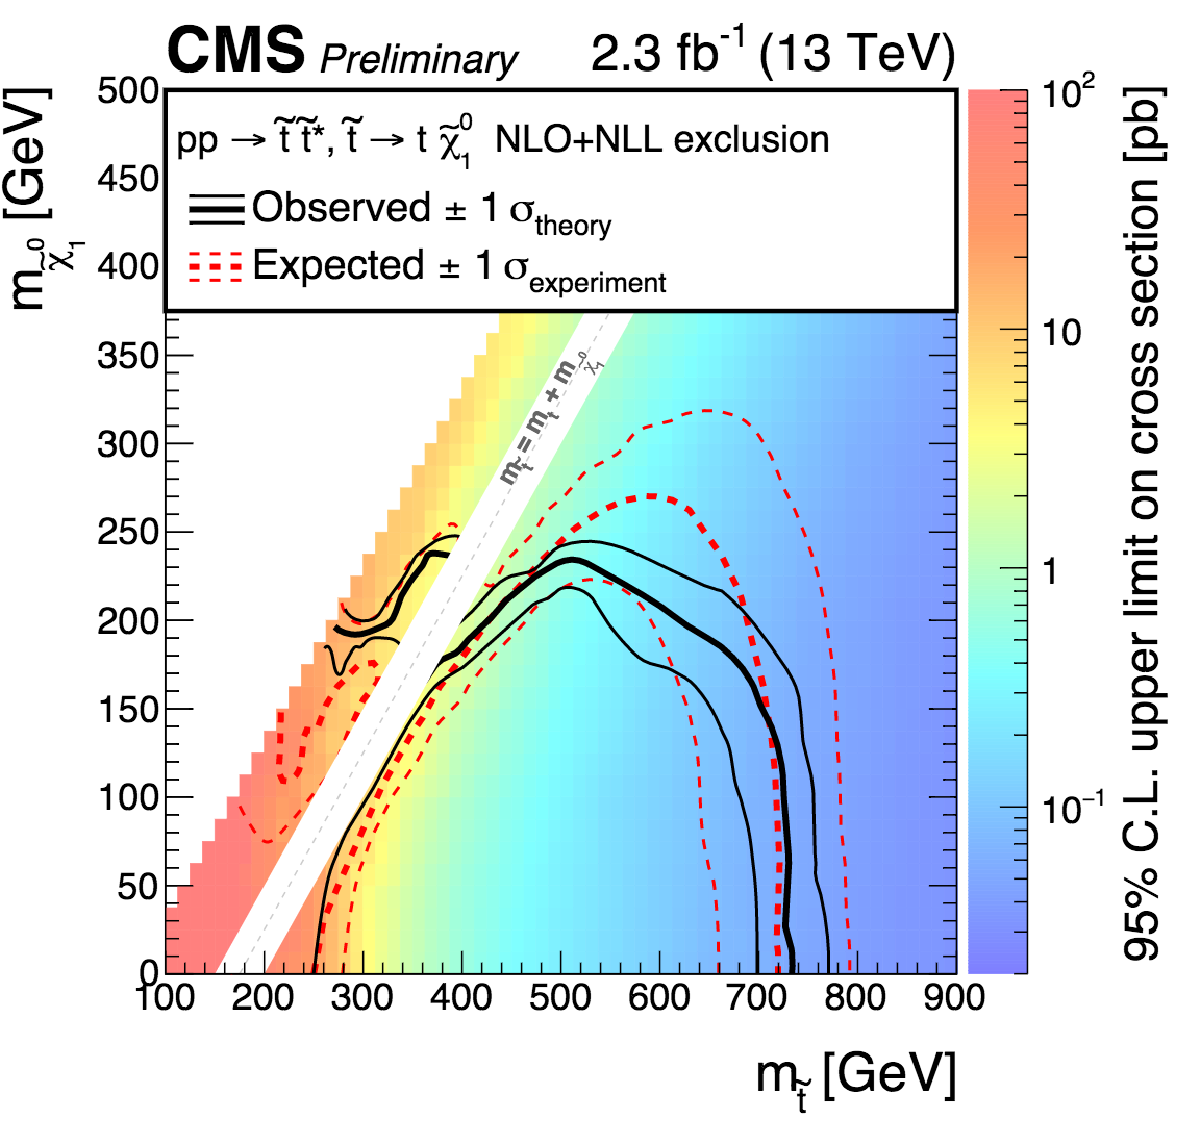
\includegraphics[width=0.4\textwidth]{1lstop/T2tt_limits.pdf}
%% \end{tabular}
%% \caption{
%% \label{fig:1lstopresults}
%% Observed yields and background predictions are shown for the 1 lepton stop analysis on the left,
%% and the cross section upper limit set by these results is shown on the right.
%% }
%% \end{center}
%% \end{figure}

The next analysis is a search targeting final states with exactly one lepton~\cite{1lmj2015}, and many jets from hadronic top decay.
In this analysis, events with exactly 1 lepton in the final state are selected,
and the jets in the event ($\mathrm{R=0.4}$) are reclustered to form large-R jets ($\mathrm{R=1.2}$).
The mass of these large-R jets is then summed to form the variable \MJ\
which tends to be large for events where large mass particles decay hadronically, for example in SUSY in final states with many top quarks.
The results of this analysis are interpreted in the context of a SUSY model where gluinos are pair-produced then each decays to a \ttbar\ pair and a stable LSP,
and gluinos up to a mass of 1600 GeV are excluded.

%% \begin{figure}[!htb]
%% \begin{center}
%% \begin{tabular}{cc}
%% 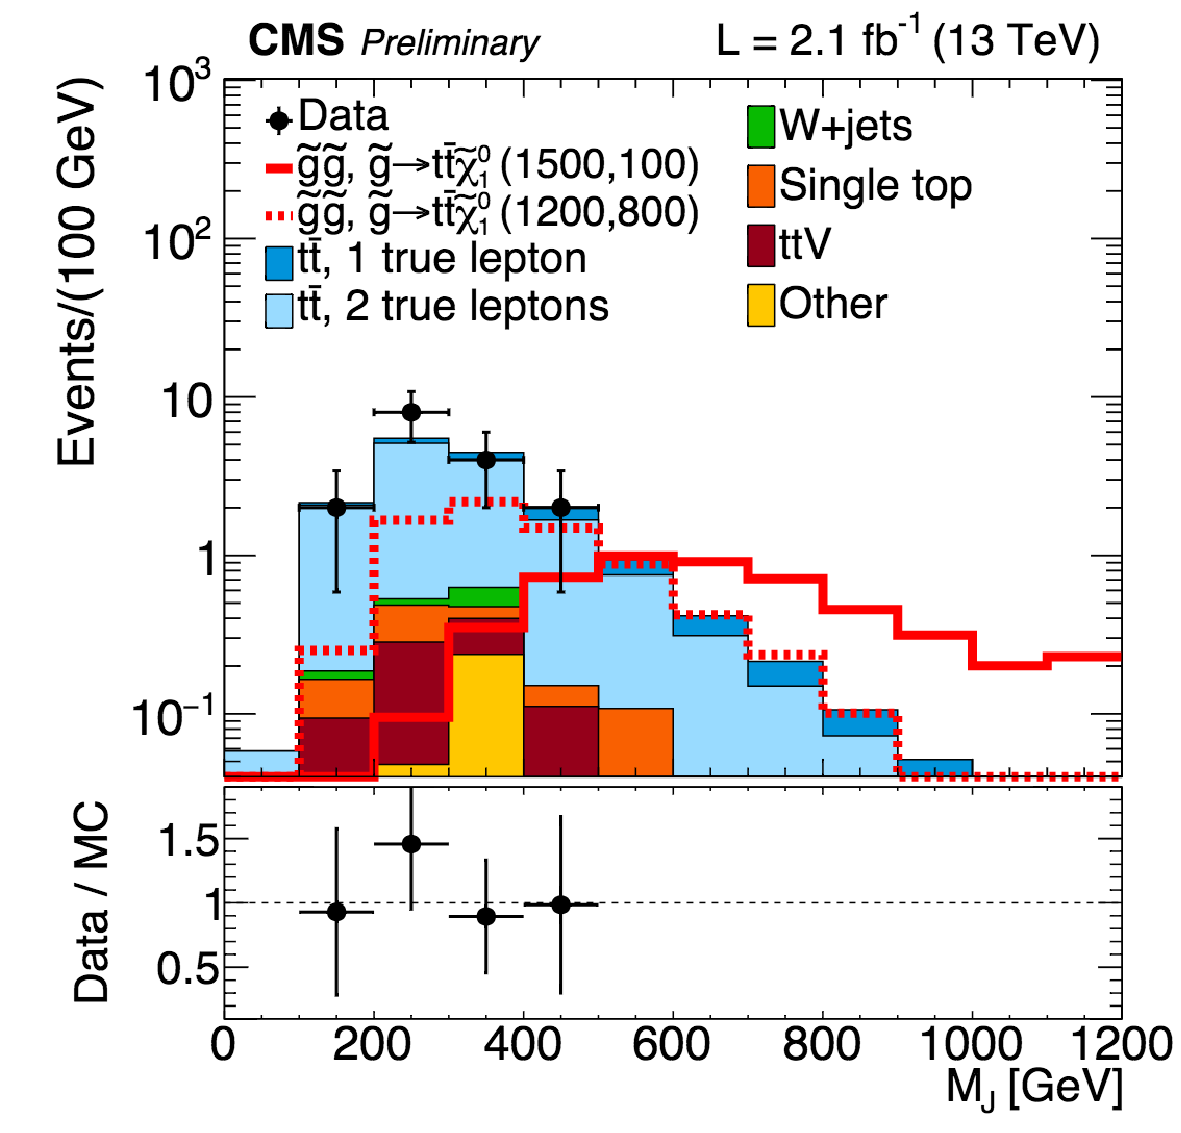
\includegraphics[width=0.4\textwidth]{1lmjet/MJ.pdf} &
%% 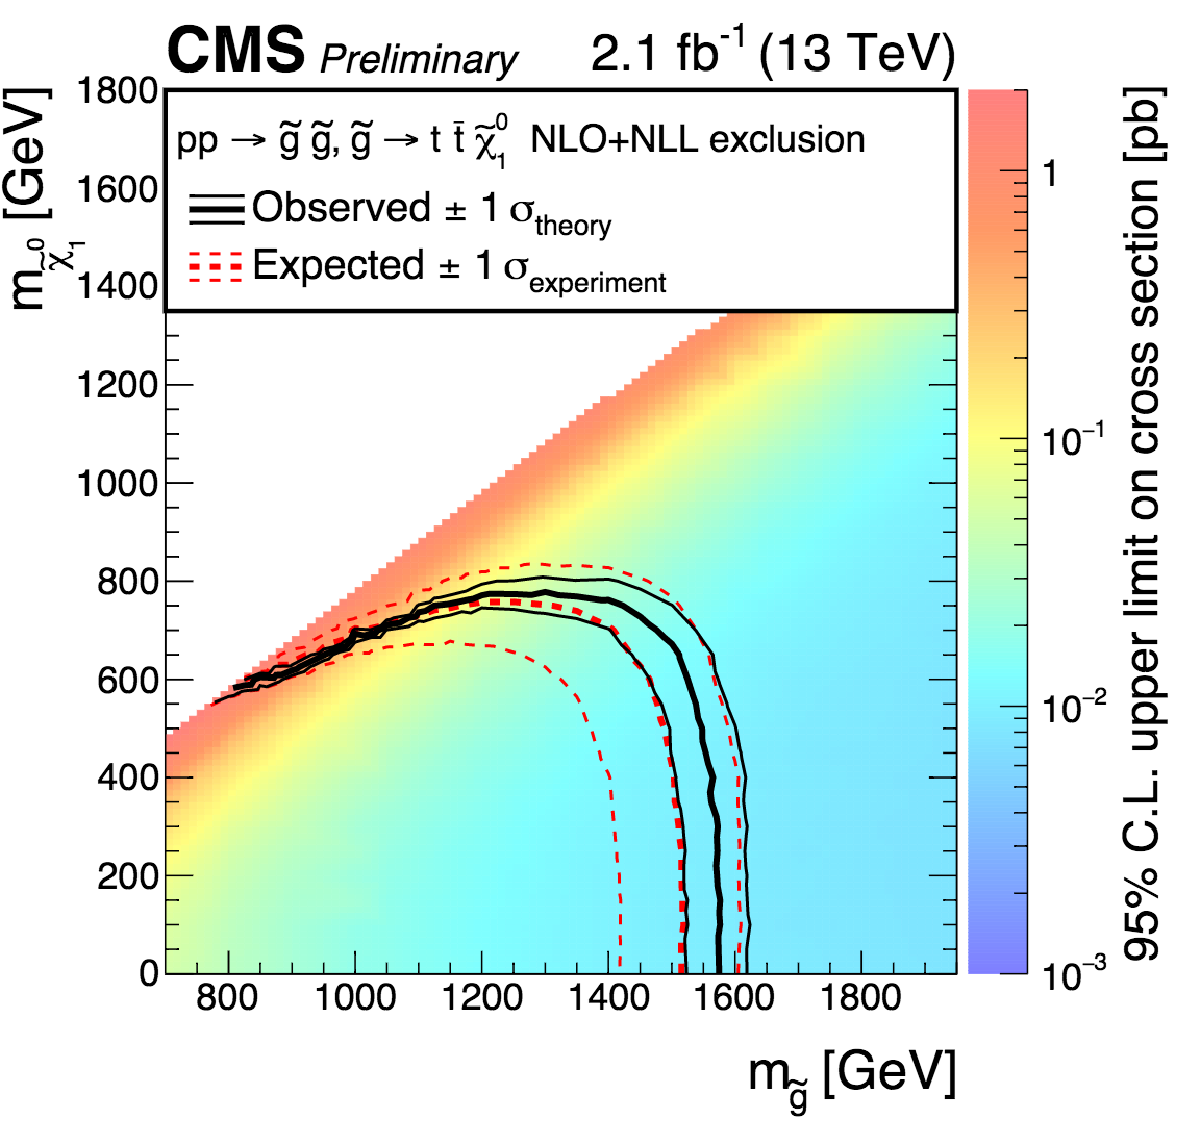
\includegraphics[width=0.4\textwidth]{1lmjet/T1tttt_limits.pdf}
%% \end{tabular}
%% \caption{
%% \label{fig:1lmjetresults}
%% Observed yields and background predictions are shown for the \MJ\ analysis on the left,
%% and the cross section upper limit set by these results is shown on the right.
%% }
%% \end{center}
%% \end{figure}


The final analysis with exactly one lepton~\cite{1lincl2015} is an inclusive search
which uses the \dphiwl\ and \LT\ variables to suppress SM backgrounds which mostly consist of \ttbar\ and W+jets.
The search is binned in the \HT, \njets, \nbtags\ in order for the search to be inclusive as possible.
The results of the search are interpreted many SUSY scenarios, for example the same model as the \MJ\ analysis,
and this analysis is seen to have similar sensitivity when interpreting the results within the context of this simplified model.

%% \begin{figure}[!htb]
%% \begin{center}
%% \begin{tabular}{cc}
%% 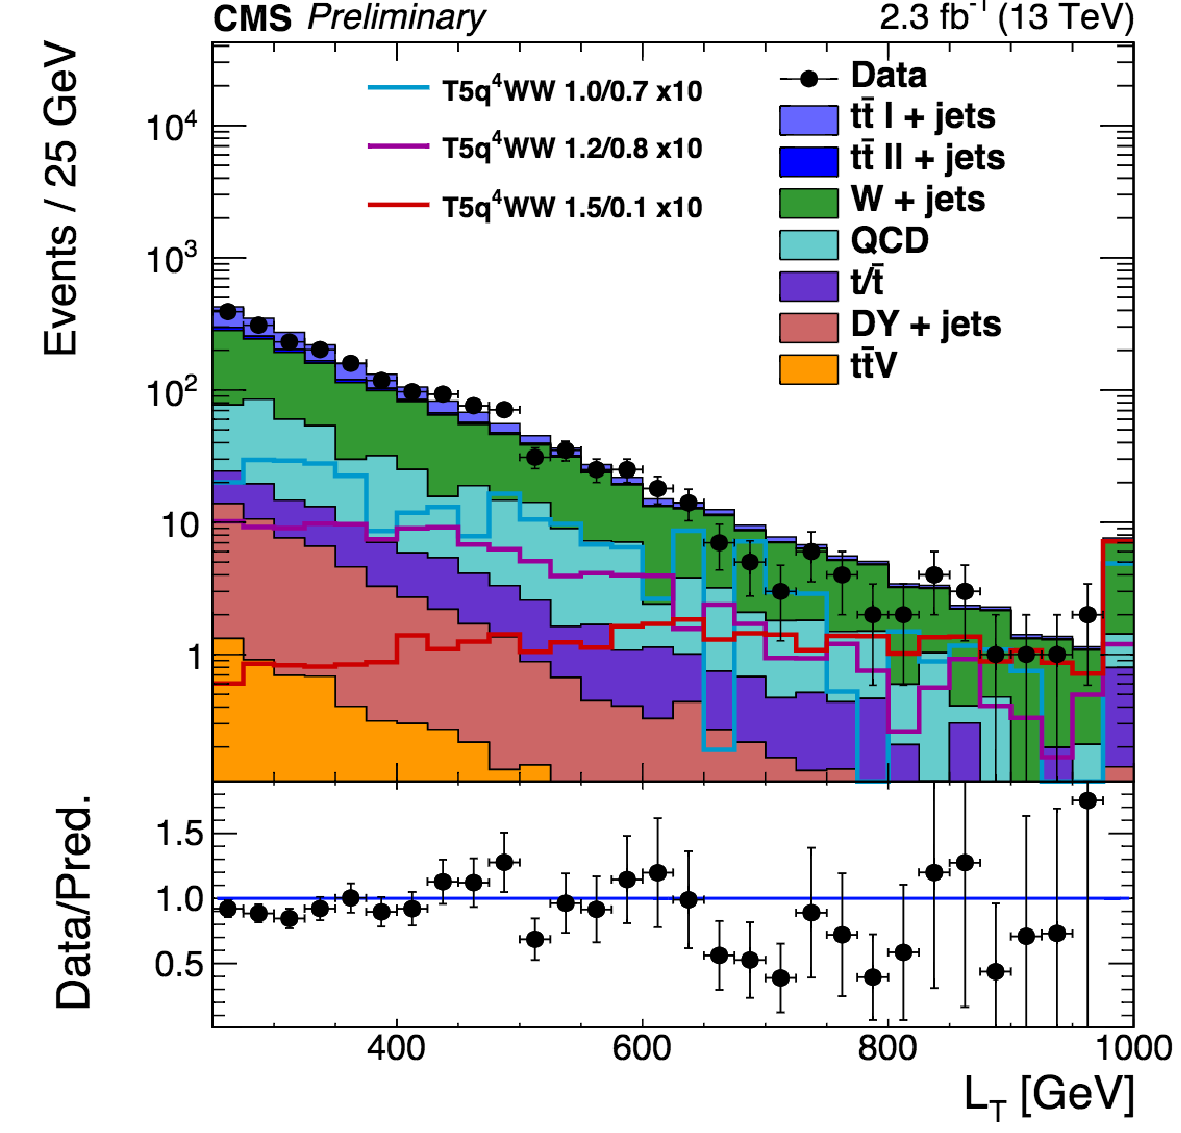
\includegraphics[width=0.4\textwidth]{1lincl/LT.pdf} &
%% 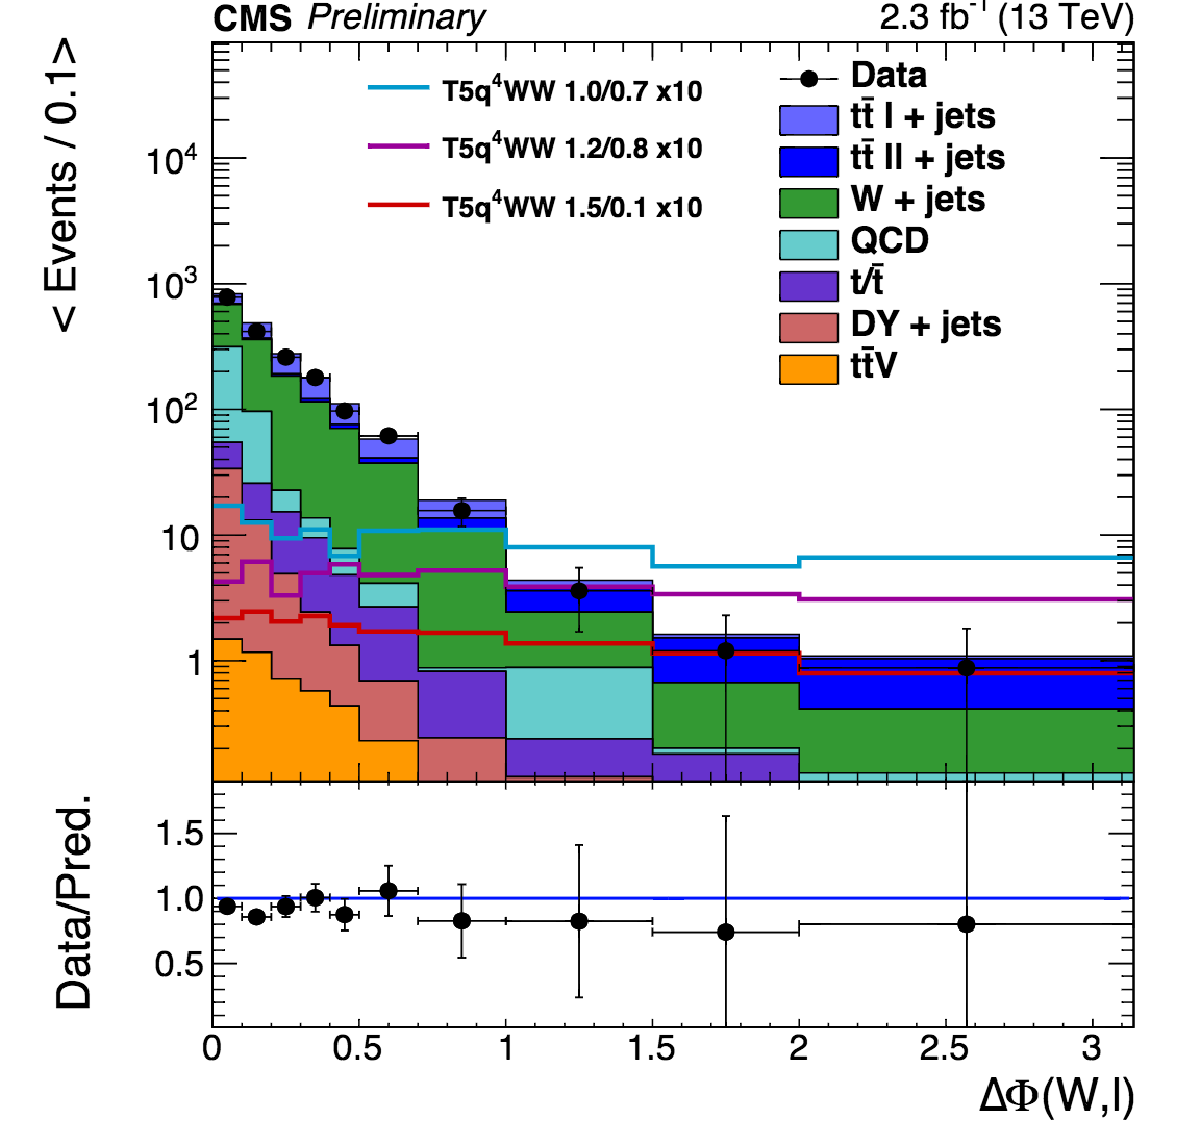
\includegraphics[width=0.4\textwidth]{1lincl/dphiWl.pdf}
%% \end{tabular}
%% \caption{
%% \label{fig:1linclresults}
%% Observed yields and background predictions are shown for the inclusive 1-lepton analysis
%% for the variables \LT\ (left) and \dphiwl\ (right).
%% }
%% \end{center}
%% \end{figure}



%% \clearpage

%% Your text comes here. Do not use sections.  For bibliography use
%% \cite{SUSYPrimer}. For figures use syntax of Fig.~\ref{fig-1}. 
%% For tables use syntax in Tab.~\ref{tab-1}. Make sure your entire
%% contribution is maximum two pages only, including references.
%% ~\cite{SUSYPrimer}
Supersymmetry (SUSY) is an extension to the standard model that can be used to
provide an explanation to some of the open problems in physics such as
a solution the hierarchy problem using stop quarks,
as well as providing potential candidates for dark matter.
Searches for SUSY are performed by the CMS collaboration in many ways, including searching for processes with leptons (e or $\mu$) in the final state.
Simplified models are used to interpret results of these searches, and a diagram for one such models,
a gauge mediated SUSY breaking (GMSB) model with a massless gravitino as the lightest SUSY particle (LSP), is shown on the left in figure~\ref{fig:SMS_T5ZZgmsb}.
In this model, gluinos are pair produced, and then each decays to a pair of quarks and a neutralino,
which subsequently decays to a Z boson and a gravitino.
Another model showning direct stop production with one of the stops eventually
decaying to a top that decays leptonically is shown on the right in the same figure.
The results presented in these proceedings focus on direct squark and gluino production.
In all of the following results, no significant deviation from the SM was observed,
and limits are set on the upper limit of the cross section of simplified models at the 95\% level using the CLs method.

\begin{figure}[!htb]
  \begin{center}
    \begin{tabular}{cc}
      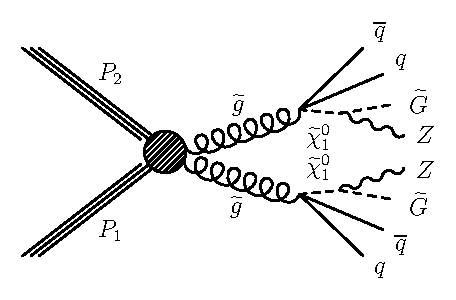
\includegraphics[width=0.4\textwidth]{intro/Feynman_graph_T5ZZgmsb.pdf} &
      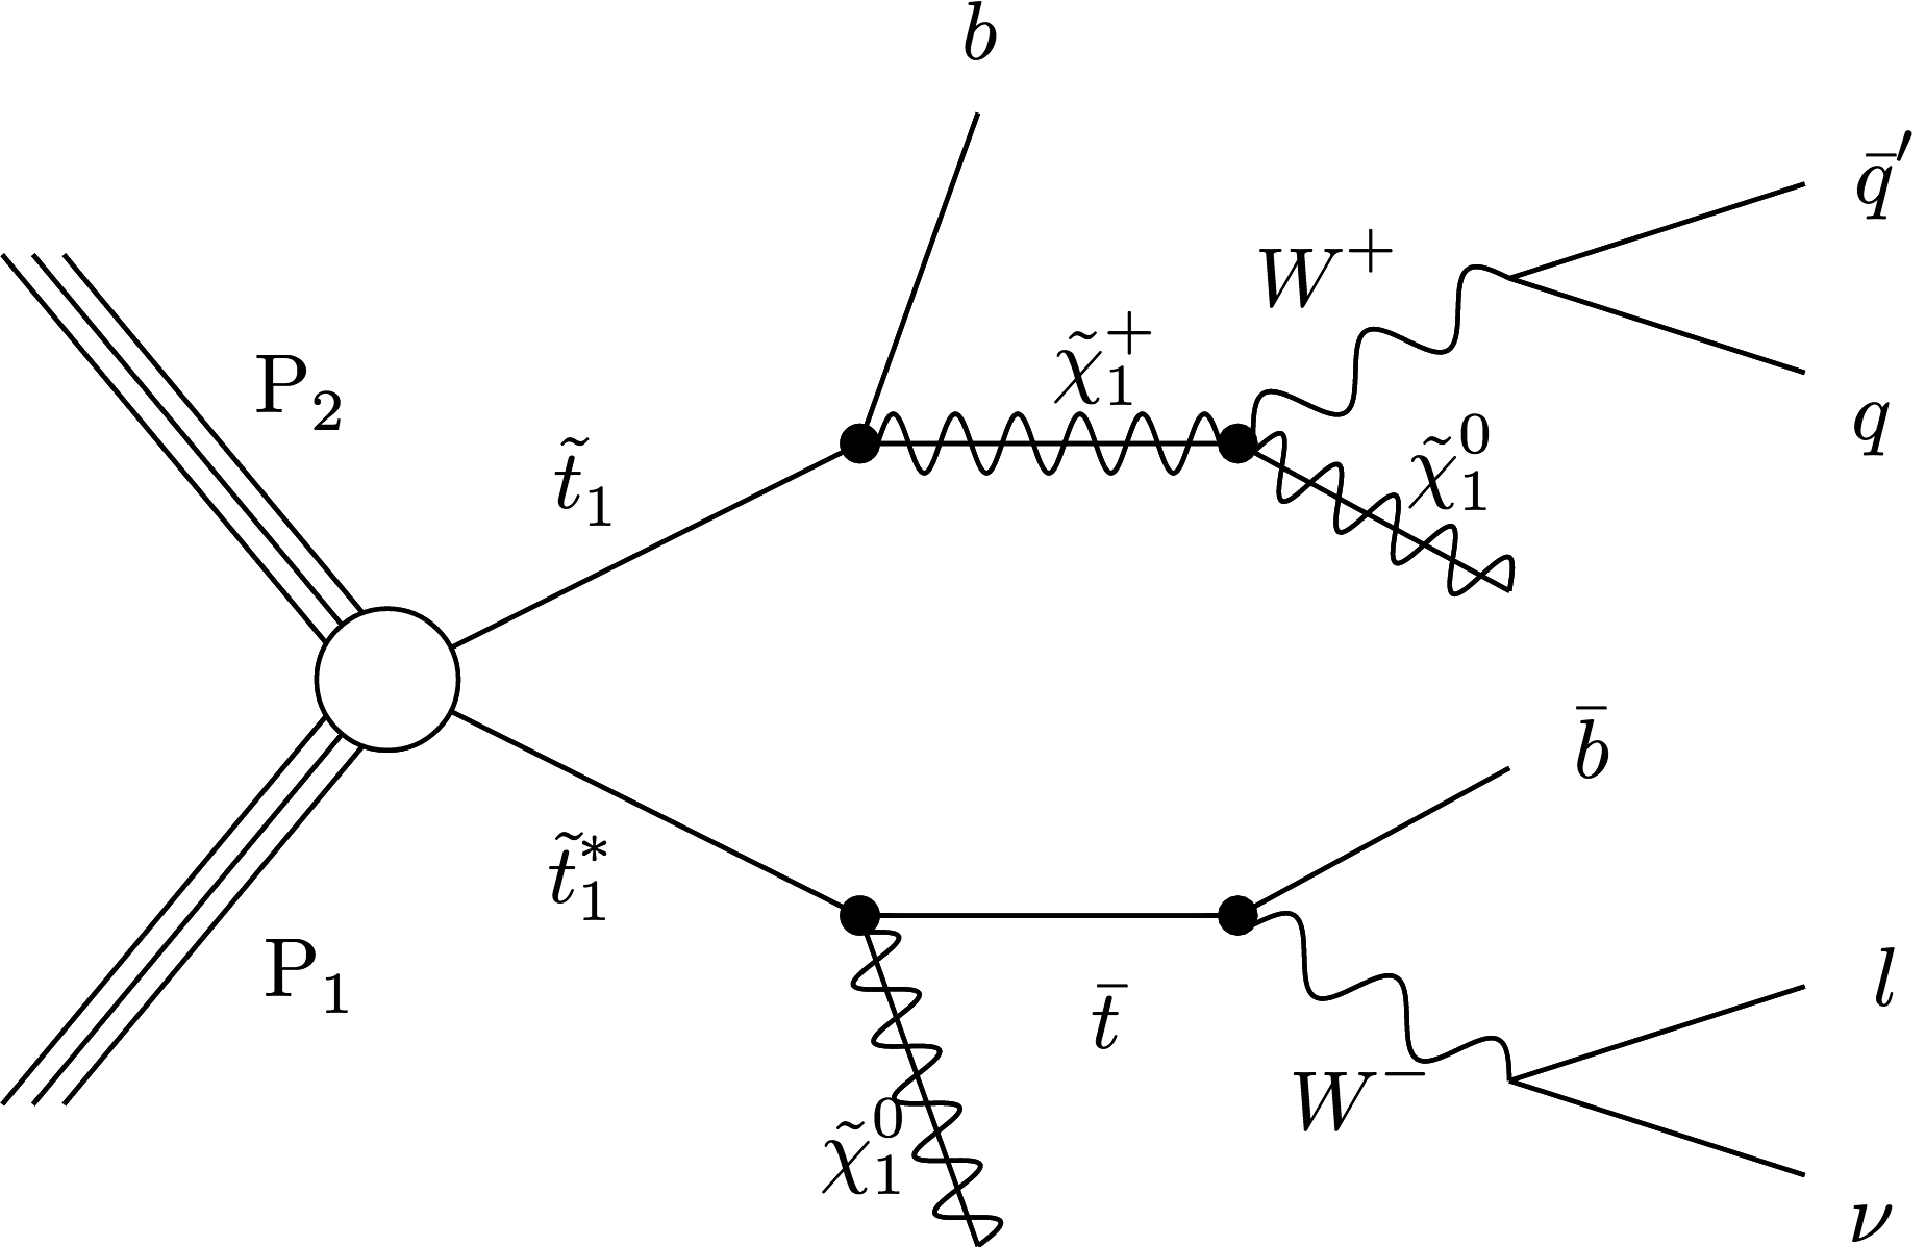
\includegraphics[width=0.4\textwidth]{intro/T2tt.pdf}
    \end{tabular}
    \caption{
      \label{fig:SMS_T5ZZgmsb}
      Diagrams showing different SUSY processes which may contain leptons in the final state are shown in this figure.
      On the left, gravitinos are pair-produced, where each eventually decays to a Z boson, two quarks, and a gravitino.
      On the right, stops are pair-produced, where one leg eventually decays to a top and a neutralino where the top decays leptonically.
    }
  \end{center}
\end{figure}

The SUSY analyses performed by CMS target a large range of topologies with varying
visible energy ($\mathrm{H_T,~M_J}$), 
invisible energy (\MET,
$\mathrm{M_T}$,
$\mathrm{M_{T2}}$,
$\mathrm{d\phi(\ell, W)}$,
$\mathrm{L_T}$),
jet multiplicity ($\mathrm{N_{jets}}$)
and flavor content ($\mathrm{N_{b-tags}}$).
The analyses are grouped by the number of leptons in the final state,
and for analyses with at least two leptons,
they are categorized according to the charge of the two leptons with the highest \pt
in same-sign, or opposite-sign final states.


%% In the analyses with exactly one lepton, three separate searches are performed.
In the first search, a search for direct stop pair production, the signal region is defined by having
exactly 1 lepton, njets, btags, and large MET.
After these cuts are made, the largest background comes from SM ttbar to dilepton, where one of the leptons is lost, leading to increased \MET.
The results of this analysis increase the sensitivity to stop production for signal models with a stop mass of 750 GeV,
which is an improvement on the previous result which was sensitive to models with a stop mass up to 650 GeV.
%% of the analysis done using data with pp collisions having an 8 TeV center of mass energy.

The next analysis is a search targeting final states with exactly one lepton, and many jets from hadronic top decay.

The final analysis with exactly one lepton, uses the dphi met W variable to discriminate background from signal.

%% 
The rest of the analyses all require at least 2 leptons in the final state.
The first analysis in this category is a search for SUSY in a final state with two same sign leptons.
This analysis is an inclusive search designed to be sensitive to many SUSY scenarios.
The baseline selection requires at least two same sign leptons with \pt\ $>$ 10-15 GeV depending on the trigger.

\begin{figure}[!htb]
\begin{center}
\begin{tabular}{cc}
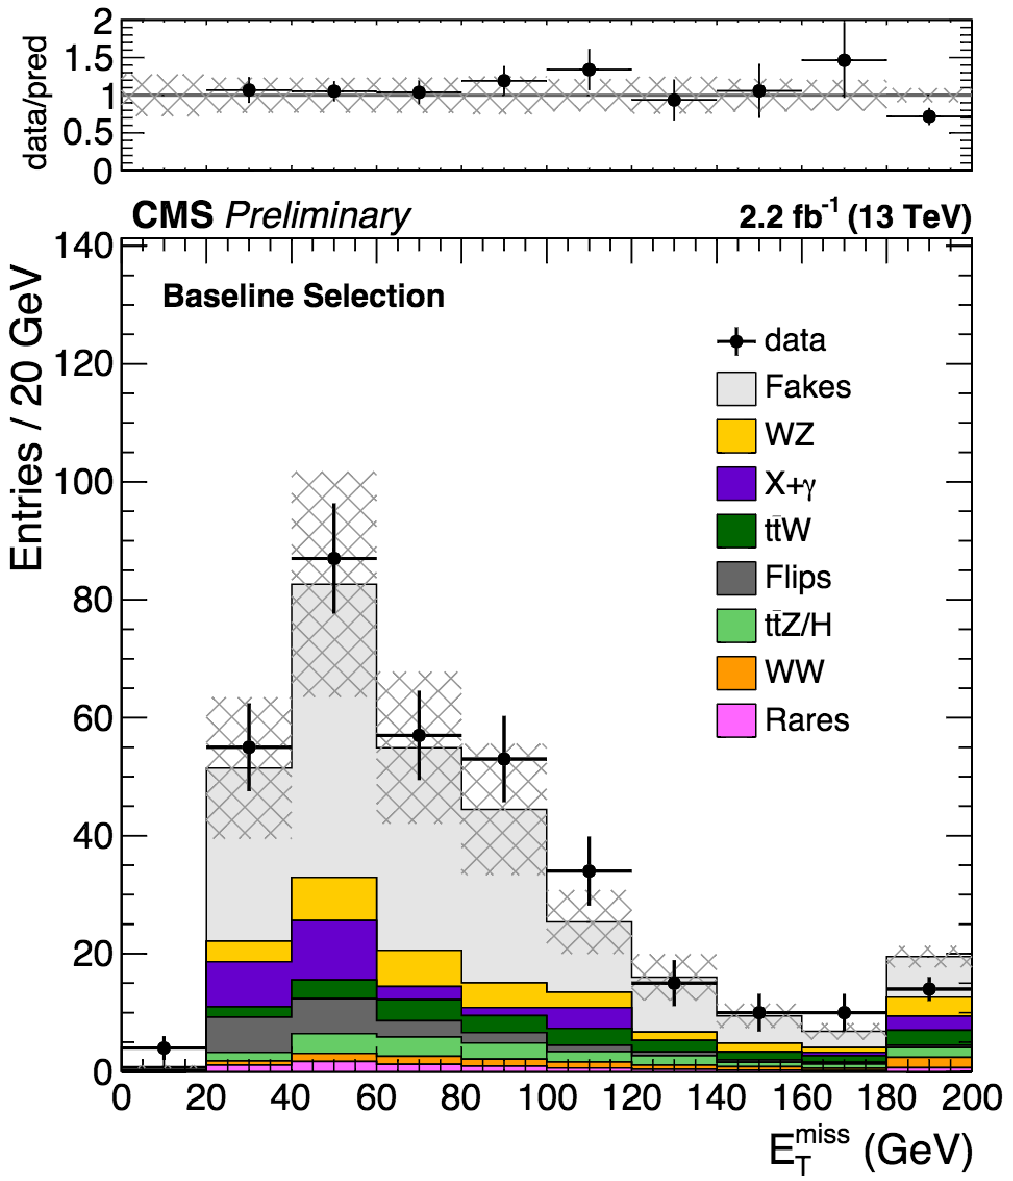
\includegraphics[width=0.4\textwidth]{2lepss/SS_MET.pdf} &
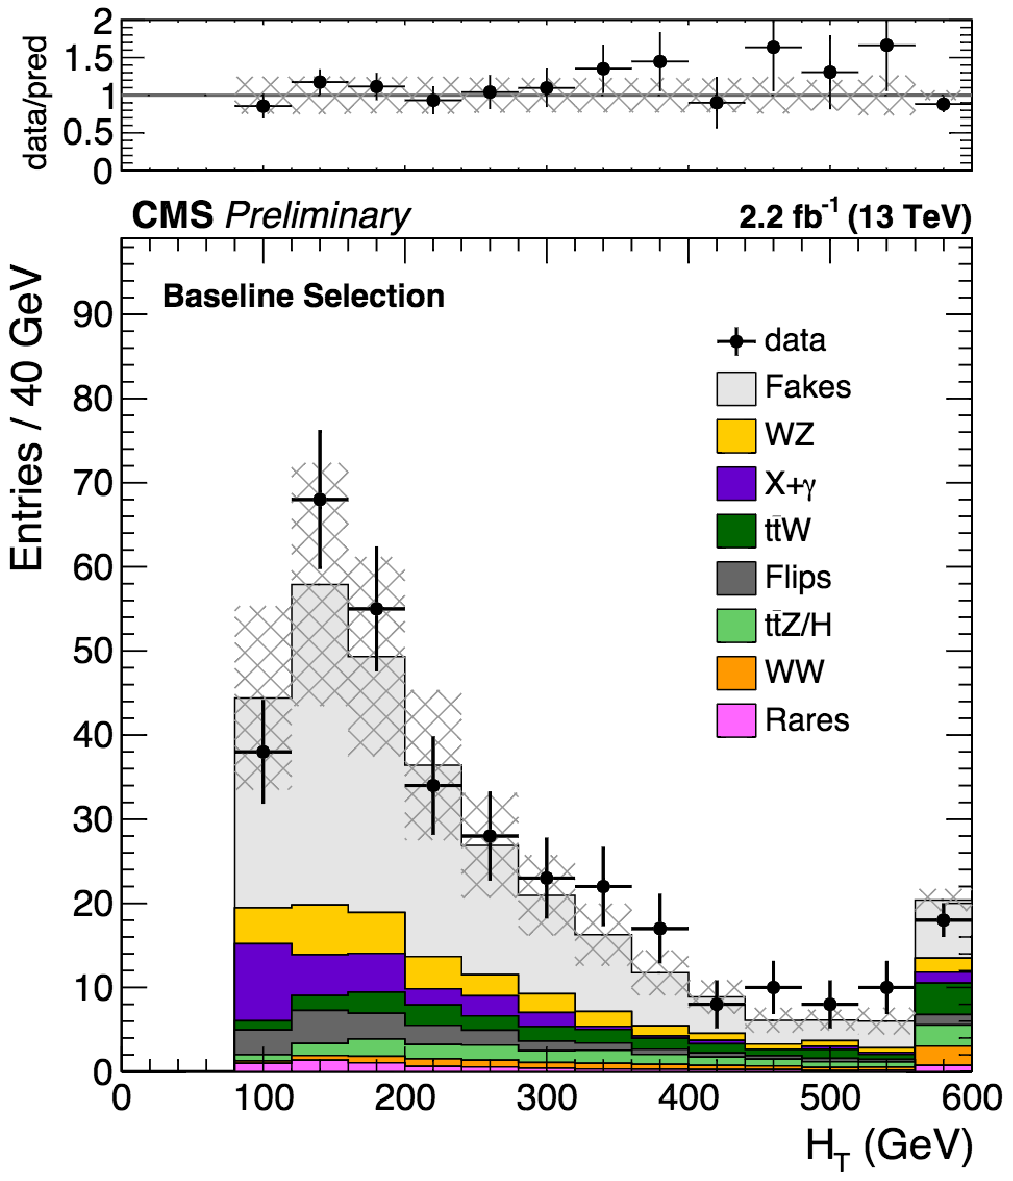
\includegraphics[width=0.4\textwidth]{2lepss/SS_HT.pdf}
\end{tabular}
\caption{
\label{fig:2lepssresults}
Observed yields and background predictions are shown for the same-sign dilepton analysis
for the variables \MET\ (left) and \HT\ (right).
}
\end{center}
\end{figure}


The next analysis is a search in events with three or more leptons.

The final analysis is a search in final states with at least two opposite-sign same-flavor leptons.
In this final state, two separate excesses were seen in run I.
CMS saw an excess in events with Mll 20-70 GeV with a significance of 2.6 sigma where ATLAS saw no excess,
and ATLAS observed a 3 sigma excess in events with two leptons with Mll 81-101, at least large HT, and large MET,
and the result from CMS in a similar signal region showed no significant deviation from the SM prediction.



The rest of the analyses all require at least 2 leptons in the final state~\cite{ssdilep2015}.
The first analysis in this category is a search for SUSY in a final state with two same sign leptons.
The baseline selection requires at least two same sign leptons with \pt\ $>$ 10-15 GeV depending on the trigger, \MET\ $>$ 50 GeV.
The analysis is then binned in \HT, \njets\ and \nbtags.
The largest background in this analysis comes from fake lepton signatures in the detector,
and a data-driven method was developed to predict this background which ends up with an uncertainty of about 40\%.

%% \begin{figure}[!htb]
%% \begin{center}
%% \begin{tabular}{cc}
%% 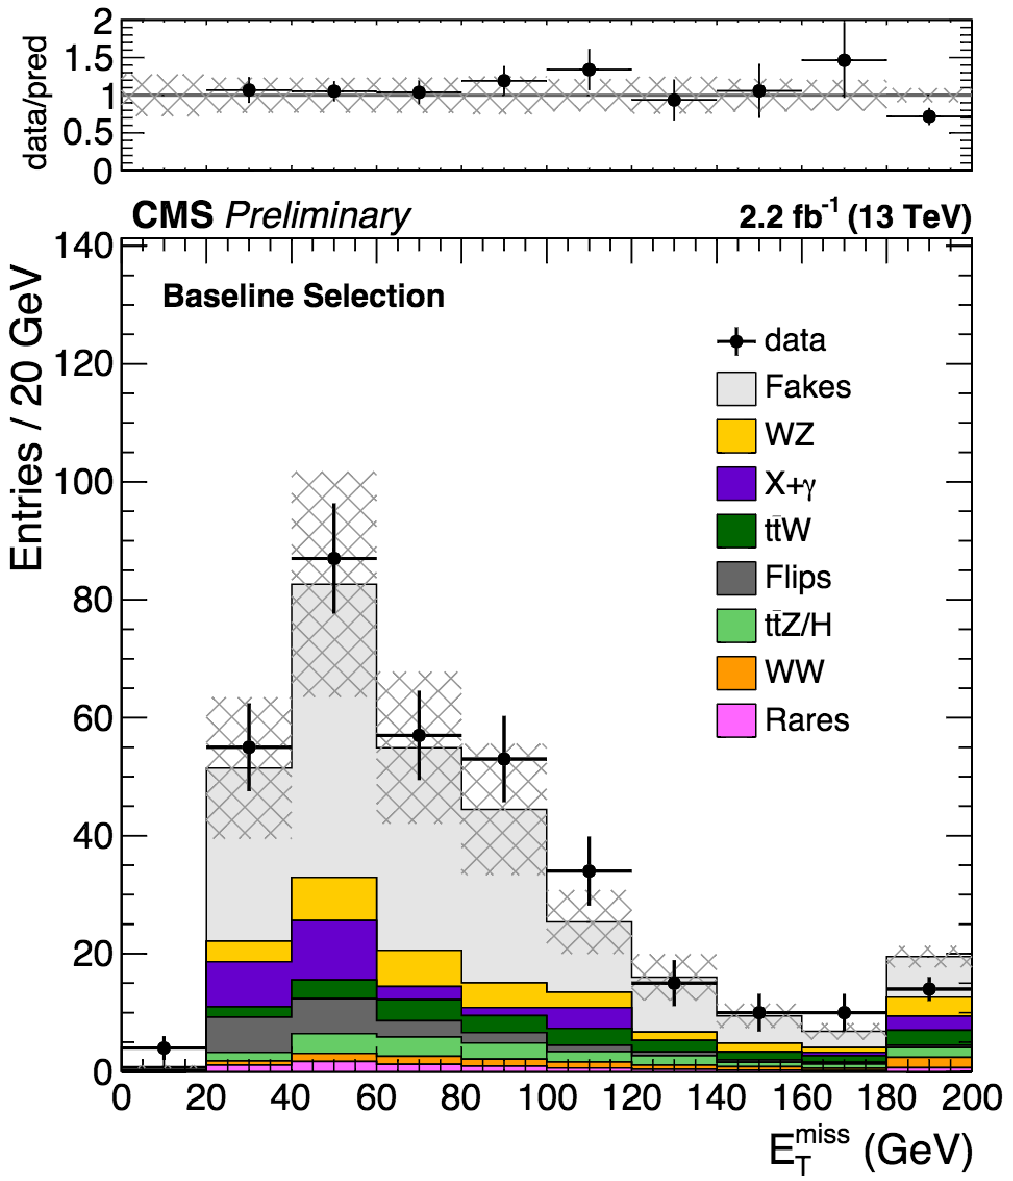
\includegraphics[width=0.4\textwidth]{2lepss/SS_MET.pdf} &
%% 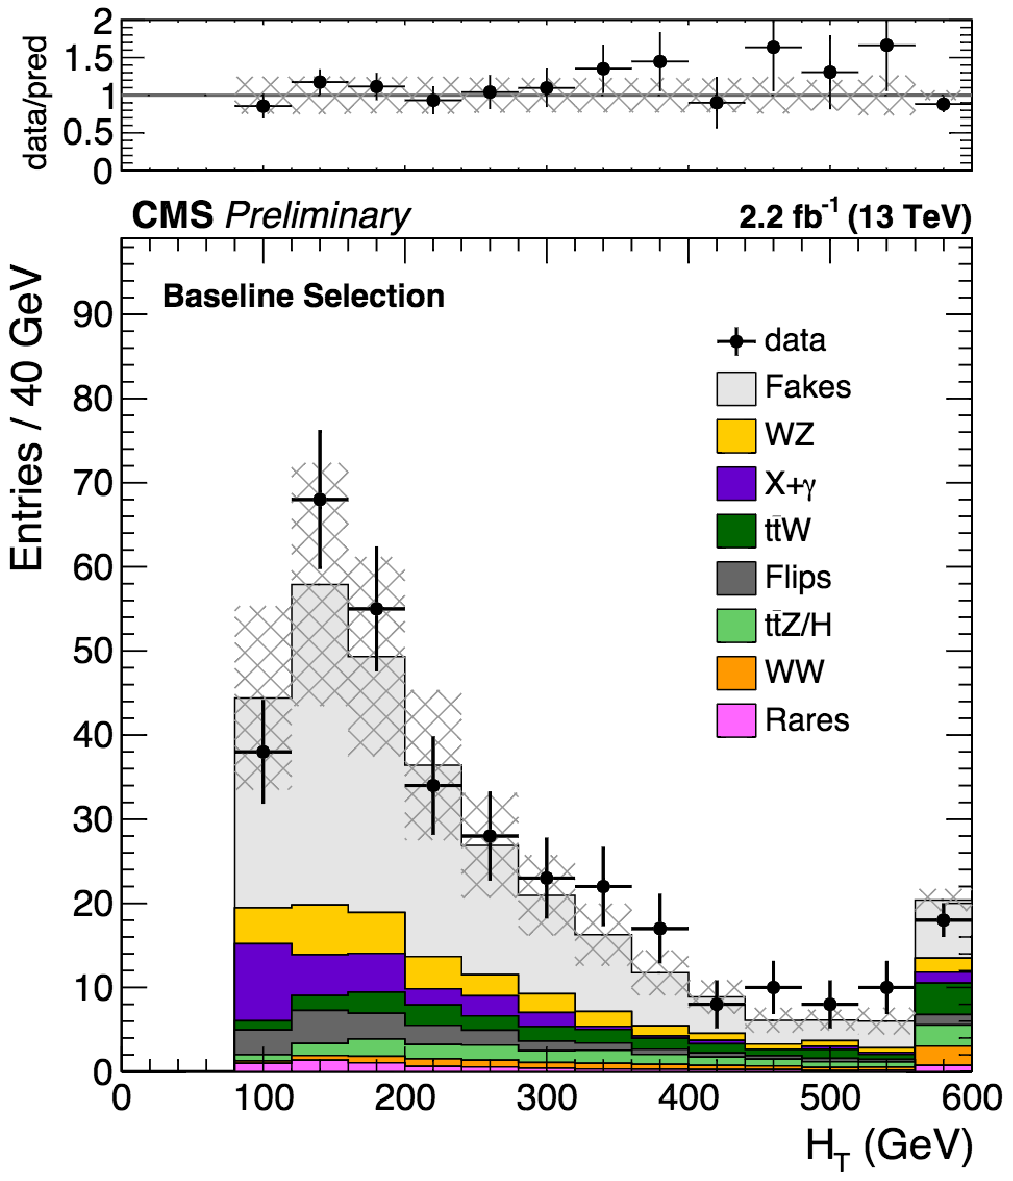
\includegraphics[width=0.4\textwidth]{2lepss/SS_HT.pdf}
%% \end{tabular}
%% \caption{
%% \label{fig:2lepssresults}
%% Observed yields and background predictions are shown for the same-sign dilepton analysis
%% for the variables \MET\ (left) and \HT\ (right).
%% }
%% \end{center}
%% \end{figure}


The next analysis is a search in events with three or more leptons~\cite{multilep2015}.
This analysis is binned in \HT, \njets\ and \nbtags,
and the largest backgrounds in the signal region comes from either SM WZ associated production,
or non-prompt leptons passing all the lepton ID requirements.

The final analysis is a search in final states with at least two opposite-sign same-flavor leptons.
Two separate excesses were observed in different \mll\ regions in run I~\cite{CMSedge,ATLASZPAPER}.
CMS saw an excess in events with \mll\ between 20-70 GeV with a significance of 2.6 $\sigma$ while ATLAS saw no excess.
ATLAS observed a 3 $\sigma$ excess in events with two leptons having \mll\ between 81-101, large \HT, and large \MET.
In the CMS analysis, a similar signal region was explored and showed no significant deviation from the SM prediction.

The analysis done by CMS was repeated in 13 TeV~\cite{osdilep2015}, and an additional signal region was added in order to search where ATLAS saw an excess at 8 TeV.
No significant excess was seen in either region where an excess was reported in 8 TeV, and the result of this analysis can be seen in figure~\ref{fig:2leposresults}.

\begin{figure}[!htb]
\begin{center}
\begin{tabular}{cc}
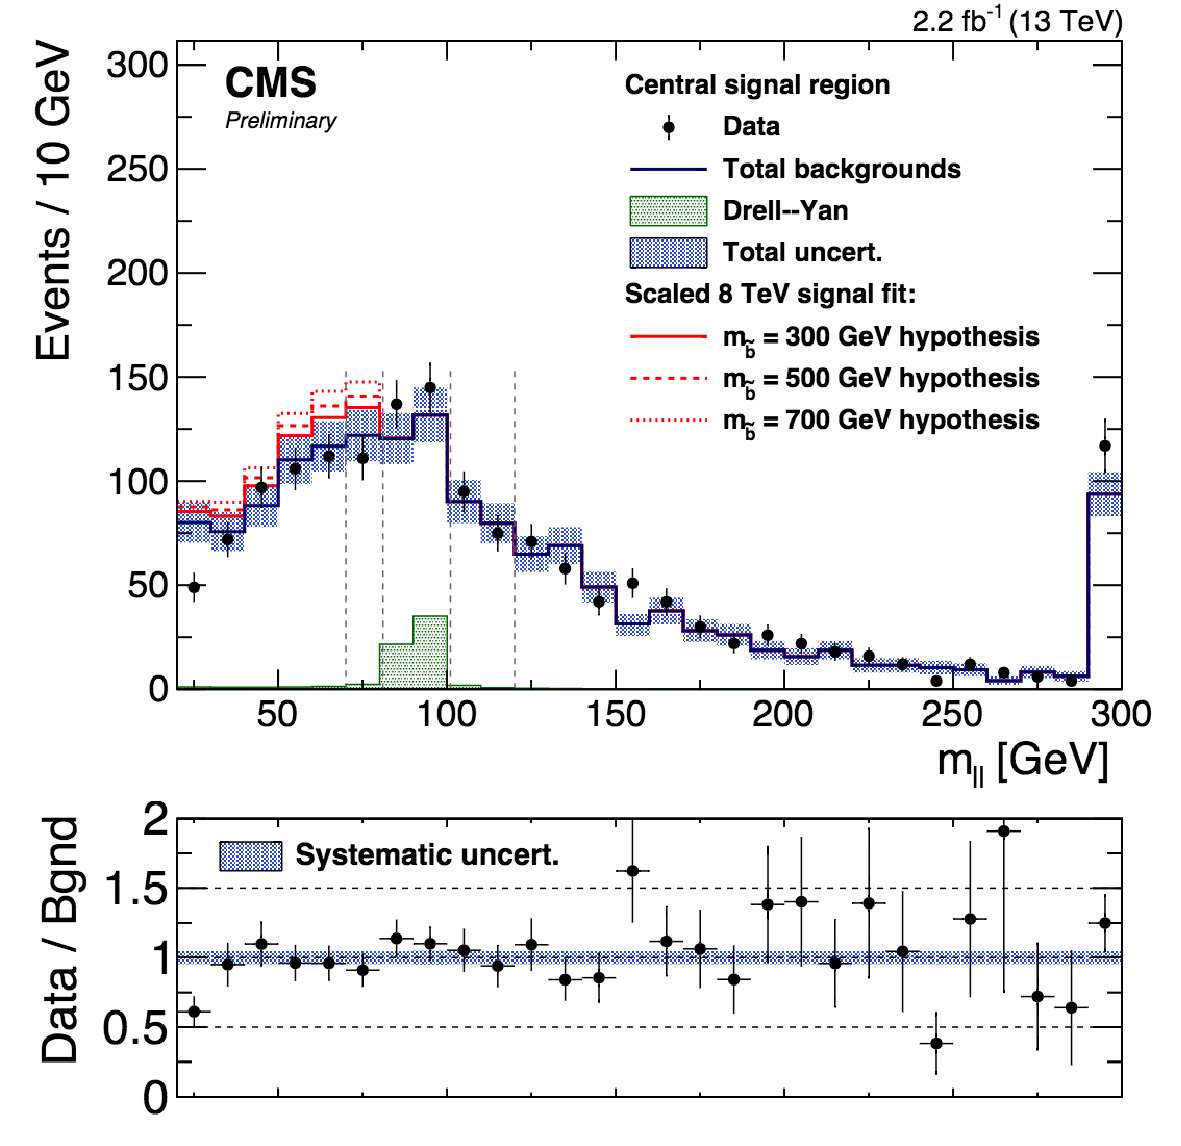
\includegraphics[width=0.4\textwidth]{edge_mll.pdf} &
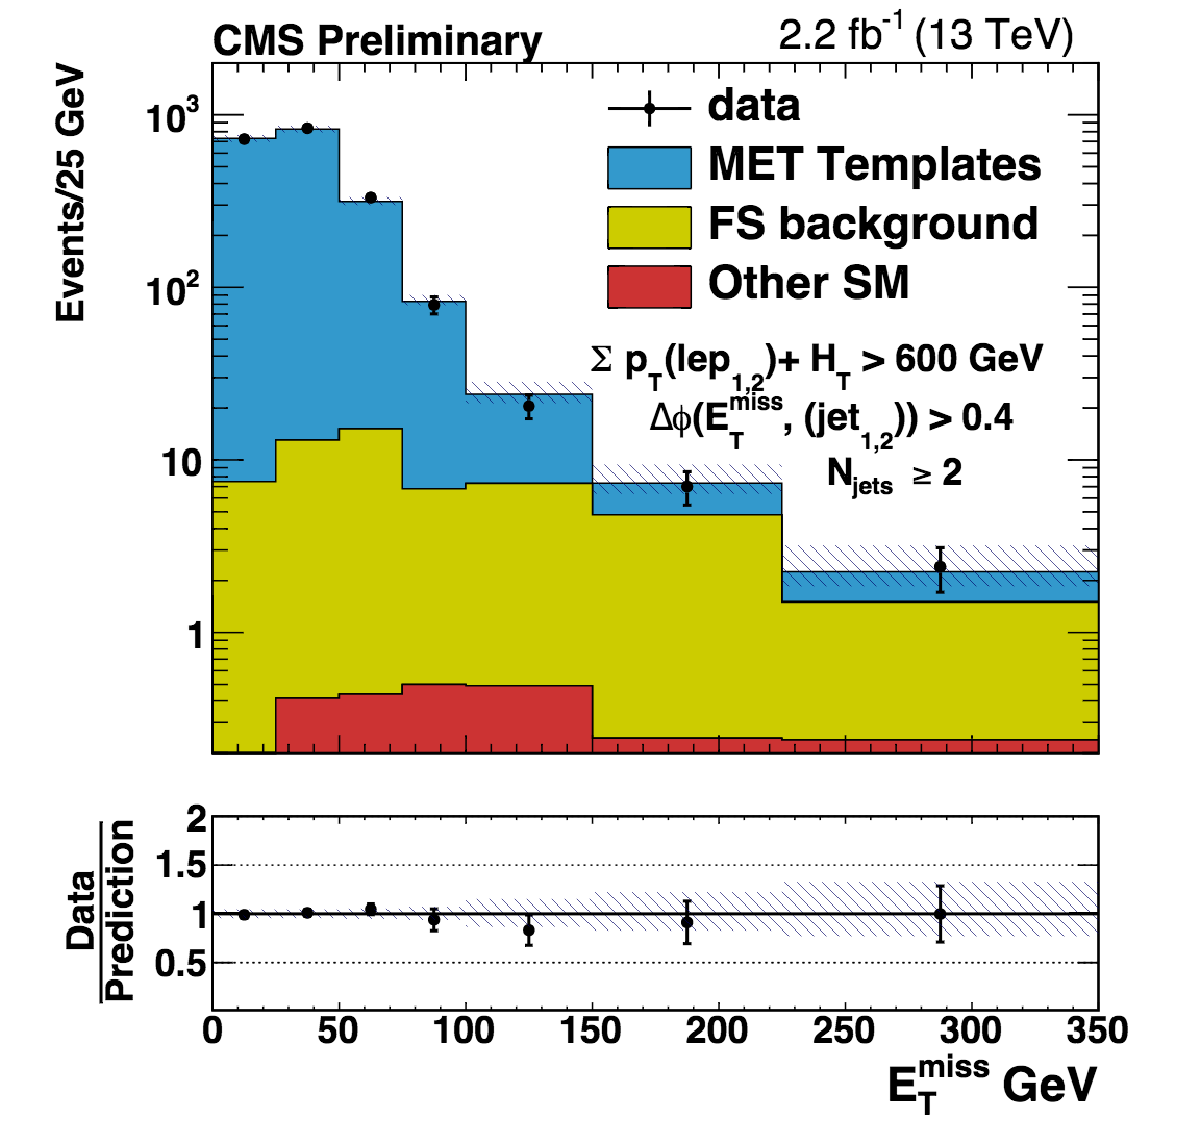
\includegraphics[width=0.4\textwidth]{MET_ATLAS_SR.pdf}
\end{tabular}
\caption{
\label{fig:2leposresults}
Observed yields and background predictions are shown for the ``edge'' signal regions (left) and ATLAS-like on Z signal region (right).
}
\end{center}
\end{figure}


%% Conclusion



% BibTeX users please use 
\bibdata{refs}
\bibliographystyle{ieeetr.bst}
\bibliography{refs}

%

%% % Non-BibTeX users please use
%% \begin{thebibliography}{}
%% %
%% % and use \bibitem to create references.
%% %
%% \bibitem{mycitation}
%% % Format for Journal Reference
%% Journal Author, Journal \textbf{Volume}, page numbers (year)
%% % Format for books
%% \bibitem{othercitation}
%% Book Author, \textit{Book title} (Publisher, place, year) page numbers
%% % etc
%% \end{thebibliography}
\end{document}
